\documentclass[a4paper, 12pt]{article}

\newcommand{\languages}{english, french}

%%%%% Tools

\usepackage{comment}
\usepackage{lipsum}
\usepackage{xstring}

%%%%% Document

\usepackage{hyperref}
\usepackage{geometry}
\usepackage{fancyhdr}
\usepackage[parfill]{parskip}

\geometry{paper=a4paper,top=3.5cm,bottom=2.5cm,right=2.5cm,left=2.5cm}

\pagestyle{fancy}
\fancyhead[L]{}
\fancyhead[R]{\leftmark}
\fancyfoot[C]{\thepage}
\renewcommand{\headrulewidth}{0pt}

%%%%% Text

\usepackage[utf8]{inputenc}
\usepackage[T1]{fontenc}

\newlength{\mytextsize}
\makeatletter
\setlength{\mytextsize}{\f@size pt}
\makeatother

%%%%% Languages

\usepackage[\languages]{babel}

% english

\addto\captionsenglish{\def\figurename{Figure}}
\addto\captionsenglish{\def\tablename{Table}}

\newcommand{\st}{\text{s.t.}}

\IfStrEq{\languagename}{english}{
	\newcommand{\lgpreamble}{Preamble}
}

% french

\frenchbsetup{StandardLists=true}

\addto\captionsfrench{\def\figurename{Figure}}
\addto\captionsfrench{\def\tablename{Tableau}}
\addto\captionsfrench{\def\proofname{Preuve}}

\newcommand{\tq}{\text{t.q.}}
\newcommand{\cad}{c.-à-d. }
\newcommand{\Cad}{C.-à-d. }

\IfStrEq{\languagename}{french}{
	\newcommand{\lgpreamble}{Préambule}
}

%%%%% Styles

\usepackage[skip=\mytextsize]{caption}
\usepackage{float}
\usepackage{mdframed}
\usepackage{enumitem}
\usepackage{eurosym}
\usepackage{color}

\newcommand\caaption[1]{\caption{#1}\vspace{-1.5\mytextsize}}

%%%%% Mathematics

\usepackage{amsmath}
\usepackage{amssymb}
\usepackage{amsfonts}
\usepackage{bm}
\usepackage{esint}
\usepackage[makeroom]{cancel}

\newcommand{\fact}[1]{#1!}
\newcommand{\deriv}{\mathrm{d}}
\DeclareMathOperator{\tr}{tr}

%%%%% SI units

\usepackage[squaren,Gray,cdot]{SIunits}
\usepackage{sistyle}

\IfStrEq{\languagename}{french}{
	\SIdecimalsign{,}
}

%%%%% Chemistry

\usepackage[version=4]{mhchem}

%%%%% Table & Figure

\usepackage{array}
\usepackage{tabularx}
\usepackage{multirow}
\usepackage{multicol}
\newcolumntype{M}[1]{>{\centering\arraybackslash}m{#1}}
%\setlength\extrarowheight{0em}
\renewcommand{\arraystretch}{1.3}

\usepackage{pgfplots}
\usepackage{tikz}
\usetikzlibrary{shapes.geometric, positioning}
\usepackage{graphics}
\usepackage{graphicx}
\pgfplotsset{axis on top, compat = 1.3}

%%%%%% Theorems and Definitions

\usepackage{amsthm}
\usepackage{thmtools}

\IfStrEq{\languagename}{english}{
	\newcommand{\lgthm}{Theorem}
	\newcommand{\lglem}{Lemma}
	\newcommand{\lgprop}{Proposition}
	\newcommand{\lgdefn}{Definition}
	\newcommand{\lghyp}{Hypothesis}
	\newcommand{\lgquest}{Question}
	\newcommand{\lgansw}{Answer}
	\newcommand{\lgexpl}{Example}
	\newcommand{\lgrmk}{Remark}
	\newcommand{\lgnote}{Note}
	\newcommand{\lgtip}{Tip}
}

\IfStrEq{\languagename}{french}{
	\newcommand{\lgthm}{Théorème}
	\newcommand{\lglem}{Lemme}
	\newcommand{\lgprop}{Proposition}
	\newcommand{\lgdefn}{Définition}
	\newcommand{\lghyp}{Hypothèse}
	\newcommand{\lgquest}{Question}
	\newcommand{\lgansw}{Réponse}
	\newcommand{\lgexpl}{Exemple}
	\newcommand{\lgrmk}{Remarque}
	\newcommand{\lgnote}{Note}
	\newcommand{\lgtip}{Conseil}
}

\theoremstyle{plain}
\newtheorem{thm}{\lgthm}[section]
\newtheorem{lem}{\lglem}[section]
\newtheorem{prop}{\lgprop}[section]

\theoremstyle{definition}
\newtheorem{defn}{\lgdefn}[section]
\newtheorem{hyp}{\lghyp}[section]
\newtheorem{quest}{\lgquest}[]

\declaretheorem[
name=\lgansw,
qed={\lower-0.3ex\hbox{$\triangle$}},
within=quest
]{answ}

\declaretheorem[
name=\lgexpl,
qed={\lower-0.3ex\hbox{$\triangle$}},
within=section
]{expl}

\theoremstyle{remark}
\newtheorem*{rmk}{\lgrmk}
\newtheorem*{note}{\lgnote}
\newtheorem*{tip}{\lgtip}

\begingroup
\makeatletter
\@for\theoremstyle:=definition,remark,plain\do{%
	\expandafter\g@addto@macro\csname th@\theoremstyle\endcsname{%
		\addtolength\thm@preskip\parskip
	}%
}
\endgroup

%%%% Others

\renewcommand{\qedsymbol}{$\blacksquare$}

%%%%%%%%%%%%%%%%%%%

%%%%%%%%%%%%%%%%%%%

\title{\'{E}valuation du projet transversal}
\author{François \textsc{Rozet}}
\date{Avril 2018}

%%%%%%%%%%%%%%%%%%%

\usepackage{colortbl}
\usepackage{listings}

\def\lstbasicfont{\fontfamily{pcr}\selectfont}

\lstdefinestyle{MatLab}{
	language=Matlab,
	%%%%%%
	showstringspaces=false,
	extendedchars=true,
	tabsize=4,
	columns=fixed,
	%%%%%%
	breaklines=true,
	breakatwhitespace=true,
	prebreak=\space,
	%%%%%%
	basicstyle=\fontfamily{pcr}\footnotesize,
	keywordstyle=\color{blue!60!black},
	commentstyle=\itshape\color{green!40!black},
	stringstyle=\color[rgb]{.627,.126,.941},
	%%%%%%
	morekeywords={clearvars, addpath, rng, mod, ones, numel, cell, cellfun, table, fieldnames, readtable, array2table, histogram, scatter, daspect, boxplot, cdfplot, icdf, cdf, kstest2, randi, corr, cf, gap, hasIn, isIn, ks2stat},
	%%%%%%
	numbersep=0.5\mytextsize,
	numbers=left,
	numberstyle={\lstbasicfont\footnotesize},
	%%%%%%
	frame=single,
	rulecolor=\color{black},
	framexleftmargin=2\mytextsize,
	xleftmargin=2\mytextsize,
	captionpos=b,
	aboveskip=1\mytextsize,
	belowskip=1\mytextsize
}

%%%%%%%%%%%%%%%%%%%

\begin{document}
	\maketitle
	\begin{enumerate}[label=Q\arabic*.]
		\item Code soumis : \par
		\lstinputlisting[style=Matlab]{resources/matlab/submit.m}
		\item Conservation de la masse
		\item Vrai
		\item Conservation de la masse et fluide incompressible
		\item $\Delta\psi$ pour chaque noeud du domaine de calcul
		\item Un système d'équations linéaires
		\item Il s'agit d'une ligne de courant particulière
		\item $\unit{\num{0.2500}}{\squaren\meter\per\second}$
		\item \textrm{ }
		 \begin{figure}[H]
		 	\centering
		 	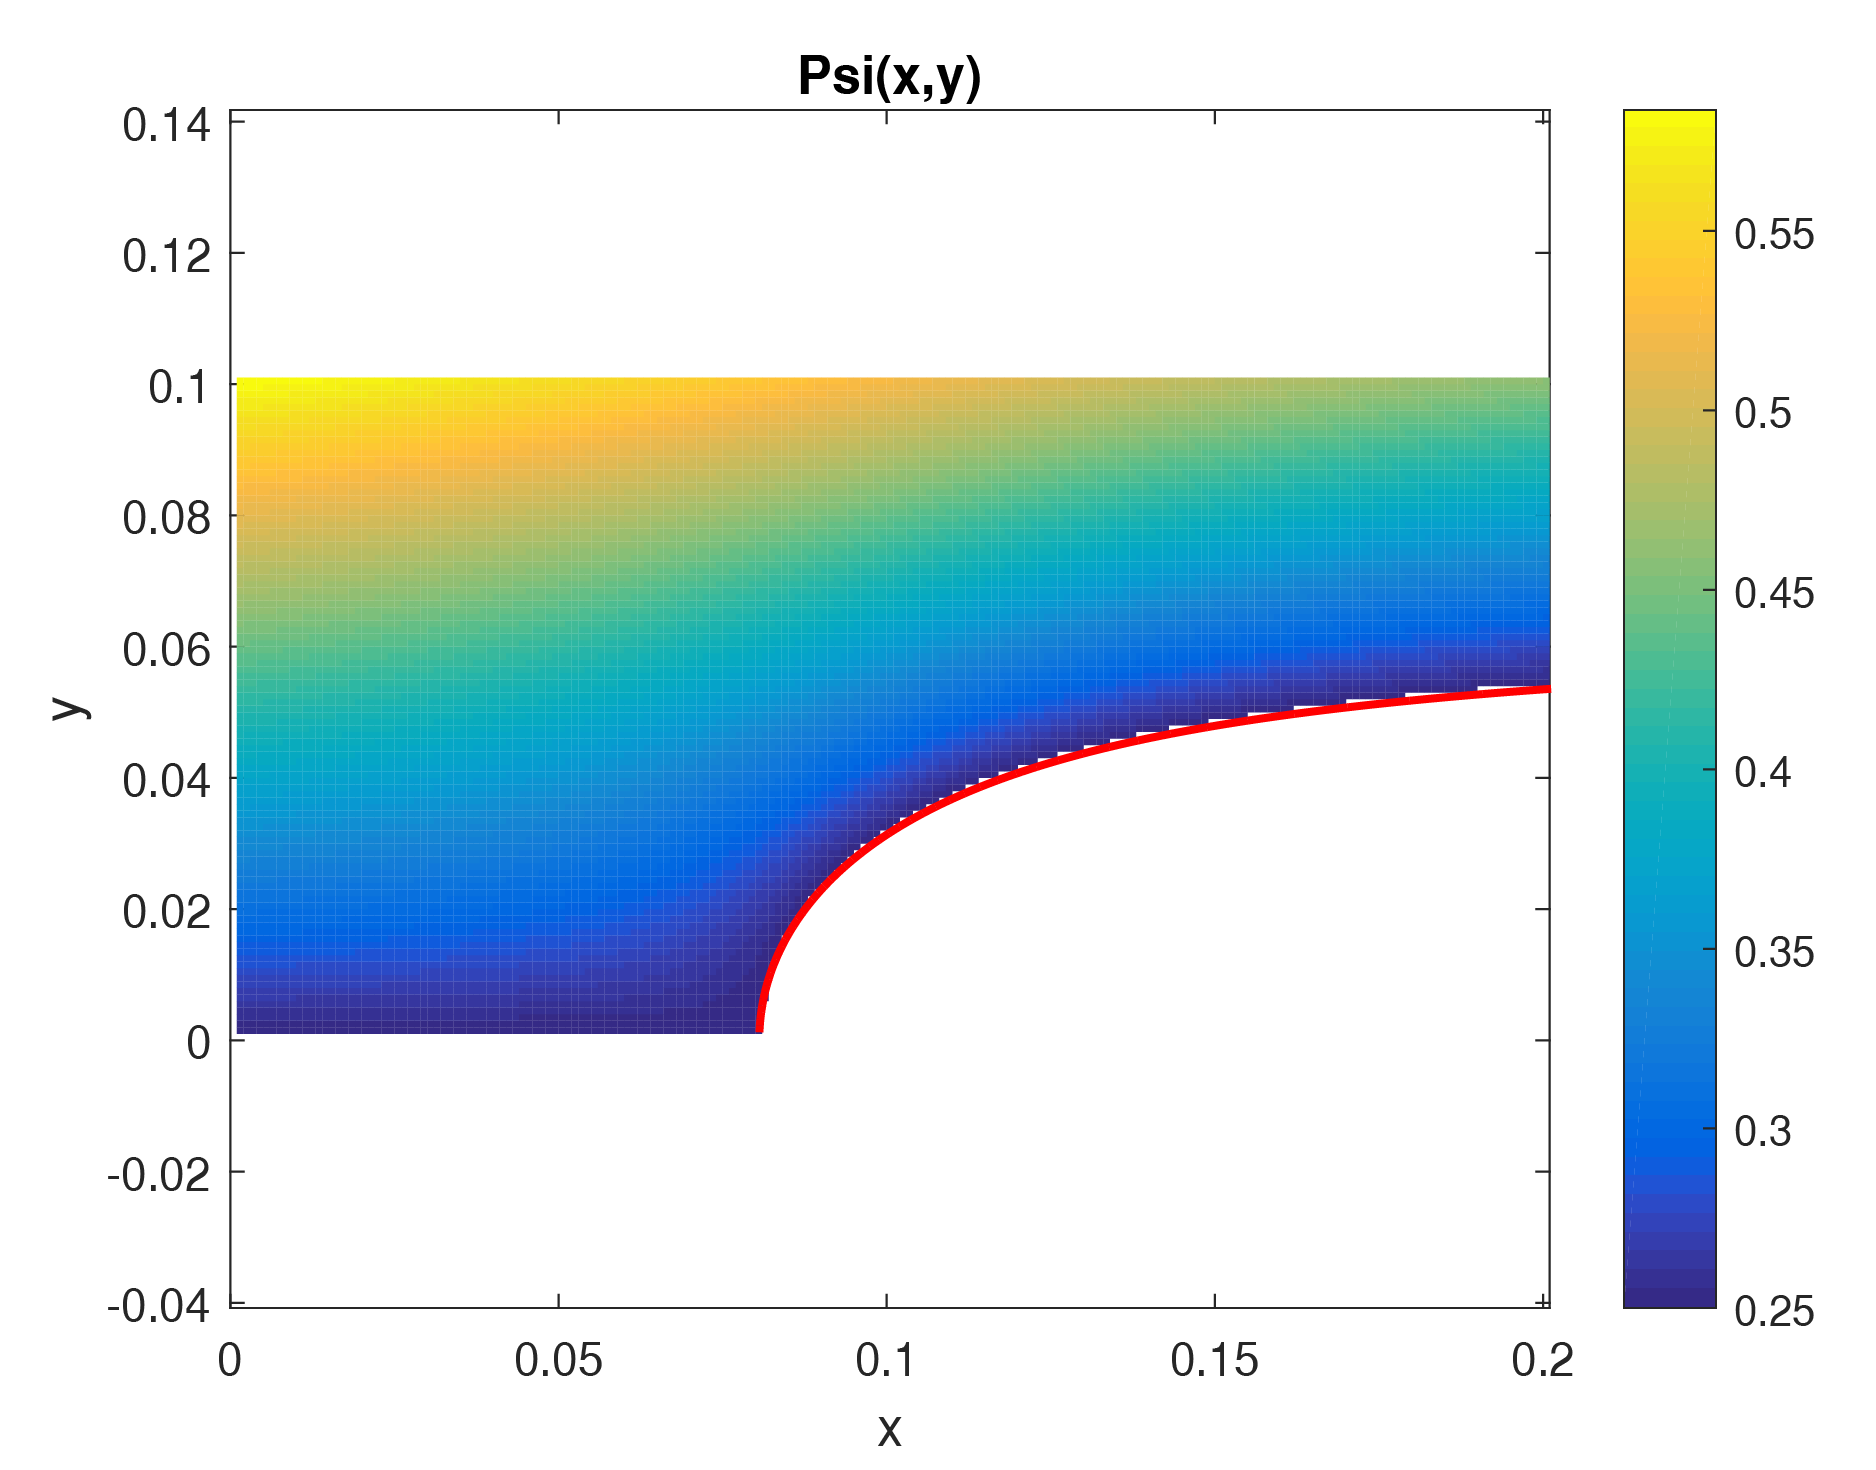
\includegraphics[scale = 0.4]{resources/png/Q9.png}
		 \end{figure}
		\item $p_\infty$
		\item $\unit{10}{\milli\meter}$
		\item \textrm{ }
		\begin{figure}[H]
			\centering
			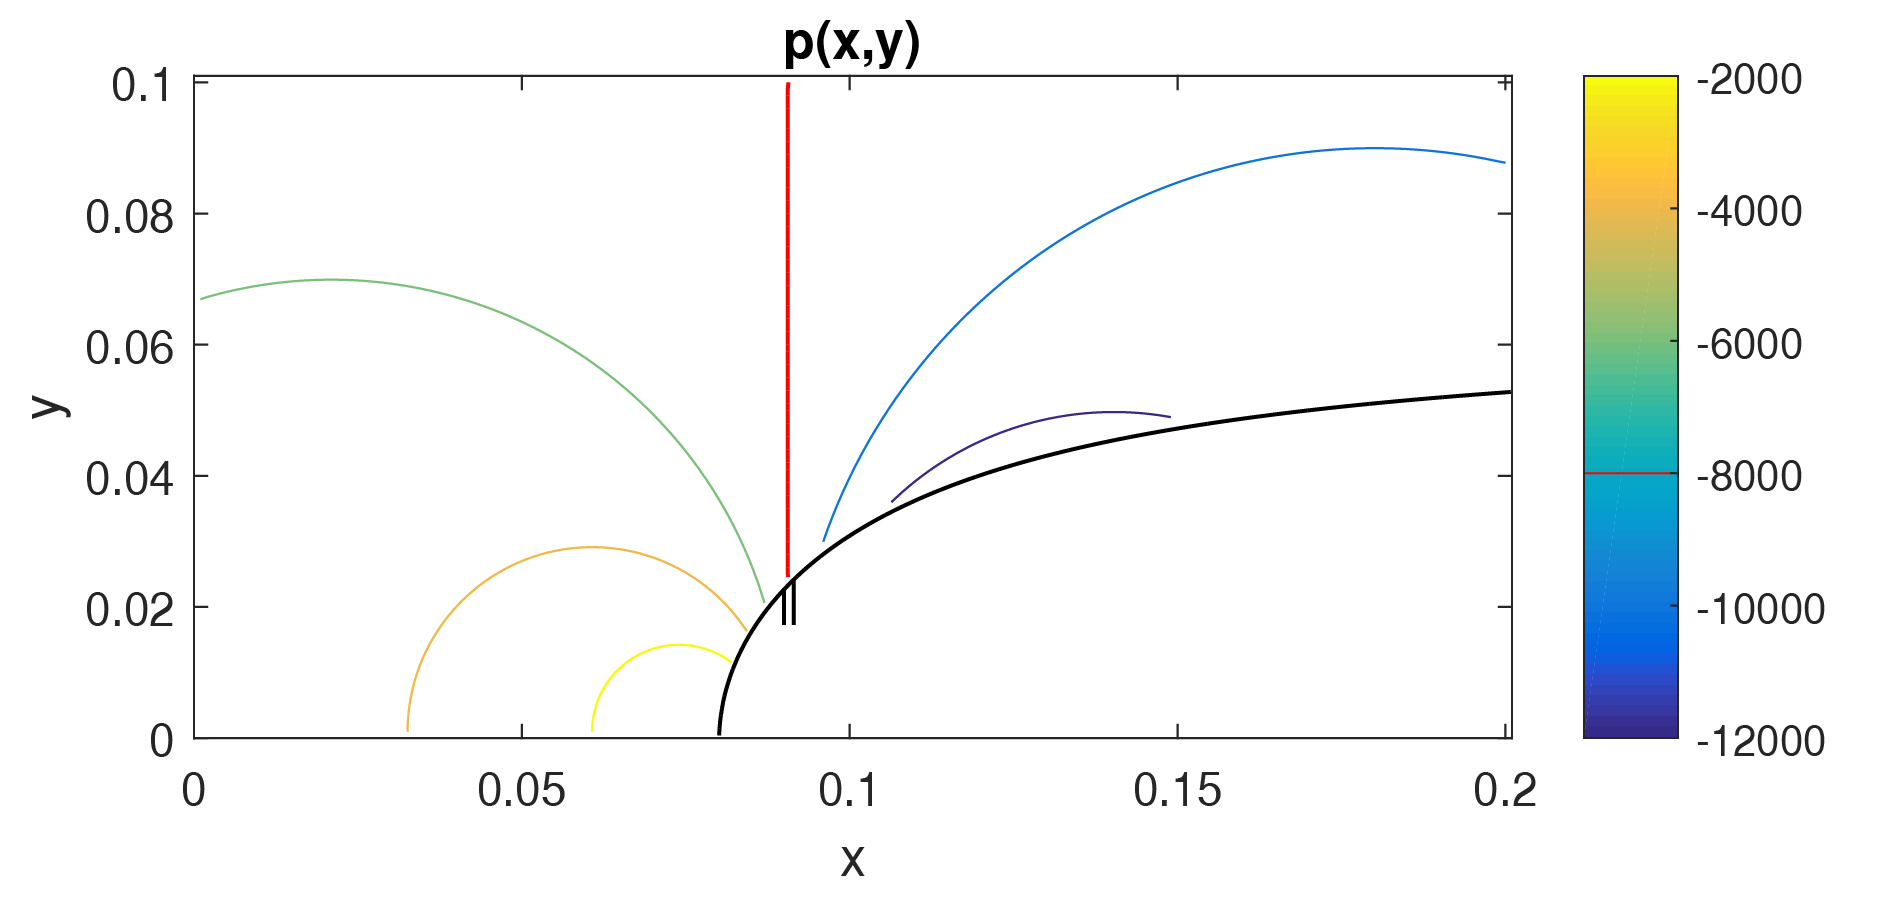
\includegraphics[scale = 0.4]{resources/png/Q12.png}
		\end{figure}
		\item
		\begin{align*}
			f                   & = \left(x - a\right)^2 + \left(y - b\right)^2 > 0 \quad \forall (x,y) \neq (a,b)                                                                                                                        \\
			u                   & = U_\infty + \frac{Q}{2 \pi} \frac{x - a}{f}                                                                                                                                                            \\
			v                   & = \frac{Q}{2 \pi} \frac{y - b}{f}                                                                                                                                                                       \\
			\Rightarrow \quad p & = C - \frac{u^2 + v^2}{2} \rho                                                                                                                                                                          \\
			                    & = C - \frac{\rho}{2} \left[\left(U_\infty + \frac{Q}{2 \pi} \frac{x - a}{f}\right)^2 + \left(\frac{Q}{2 \pi} \frac{y - b}{f}\right)^2 \right]                                                           \\
			                    & = C - \frac{\rho}{2} \left[U_\infty^2 + 2\frac{Q U_\infty}{2 \pi} \frac{x - a}{f} + \frac{Q^2}{4 \pi^2} \frac{\left(x - a\right)^2}{f^2} + \frac{Q^2}{4 \pi^2} \frac{\left(y - b\right)^2}{f^2} \right] \\
			                    & = C - \frac{\rho}{2} \left[U_\infty^2 + \frac{Q U_\infty}{\pi} \frac{x - a}{f} + \frac{Q^2}{4 \pi^2} \frac{f}{f^2}\right]                                                                               \\
			                    & = p_\infty - \frac{\rho Q U_\infty}{2 \pi} \left(x - a + \frac{Q}{4 \pi U_\infty}\right) \frac{1}{f}
		\end{align*}
		Pour l'isobare $p = p_\infty$,
		\begin{align*}
			0                       & = \frac{\rho Q U_\infty}{2 \pi} \left(x - a + \frac{Q}{4 \pi U_\infty}\right) \frac{1}{f} \\
			\Leftrightarrow \quad x & = a - \frac{Q}{4 \pi U_\infty}
		\end{align*}
		Ainsi, l'isobare est une droite verticale d'abscisse $a - \frac{Q}{4 \pi U_\infty}$. Pour nos valeurs, cette dernière est $\unit{\num{0.090552816056757}}{\meter}$ et, ainsi, la distance à la source est $\unit{\num{9.947183943243}}{\milli\meter}$. La position et la forme de l'isobare correspondent aux résultats numériques trouvés précédemment.
		\item  \unit{\num{0}}{\squaren\meter\per\second}\footnote{\unit{\num{6.895525817007808e-16}}{\squaren\meter\per\second}.}
		\item \unit{\num{1.045758122397198}}{\squaren\meter\per\second}
		\item
		\begin{itemize}
			\item Trainée îlot 1 : \unit{\num{0}}{\newton\per\meter}
			\item Trainée îlot 2 : \unit{\num{0}}{\newton\per\meter}
			\item Portance îlot 1 : \unit{\num{0}}{\newton\per\meter}
			\item Portance îlot 2 : \unit{\num{1230}}{\newton\per\meter}
		\end{itemize}
		\item Pour le premier îlot, les pressions agissant sur les faces horizontales étant sensiblement les mêmes, il est naturel que la portance soit nulle. \par 
		Au contraire, pour le second, la pression plus faible au dessus du bloc induit une portance positive dans le sens des $y$ positifs. \par
		A propos de la trainée, d'après Runge-Kutta, il ne peut pas y en avoir si il n'y a pas de circulation. Etant dans ce cas, les résultats obtenus sont justifiés.
		\item Leurs conditions aux limites sont différentes et, dès lors, le laplacien, les vitesses et les pressions le sont aussi. Puisque que la fonction \texttt{force} travaille sur les pressions, les portances et trainées ne sont pas semblables.
	\end{enumerate}	
\end{document}